
We now present \emph{symbolic pairwise lockset analysis}, a novel method for data race analysis in device drivers.  In Section~\ref{sec:symbolicpairwise} we describe how the approach works in a semi-formal manner, with respect to a simple concurrent programming model.  In Section~\ref{sec:whoopimplementation} we explain how we have implemented symbolic pairwise lockset analysis in a practical tool, \whoop, that can be applied directly to driver source code, to check whether pairs of driver entry points can race with one another.

Our experimental evaluation (Section~\ref{evaluation}) demonstrates that the \whoop technique has value as a stand-alone analyzer, and that results from \whoop can be exploited to significantly boost the performance of a more precise symbolic analysis for concurrency, based on context bounding and stratified inlining, offered by the \corral~\cite{lal2012corral} tool; we discuss the latter approach in Section~\ref{corral}.

\subsection{Symbolic Pairwise Lockset Analysis}\label{sec:symbolicpairwise}

\ADComment{Top level question about this section: is the motivation super-clear?  Is it obvious why we go for the pairwise approach?}

Our approach considers, for a given driver, every pair of entry points that can potentially execute concurrently.  For each such pair, we use symbolic verification to check whether it is possible for the pair to race in a shared variable. We soundly model the effects of additional entry points by treating the driver shared state abstractly: when an entry point reads from the shared state, a nondeterministic value is returned.  

Symbolic verification of a pair of entry points works by (i) instrumenting each entry point with additional state to record locksets, and (ii) attempting to verify a sequential program that executes the instrumented entry points in sequence and then asserts that the lockset for each shared variable is non-empty.  Verification of the resulting sequential program can be undertaken using any sound method; in practice we employ the Boogie verification engine~\cite{barnett2006boogie}, which requires procedure specifications and loop invariants to be generated, after which verification conditions are generated and discharged to an automated theorem prover.

We now detail the approach in a semi-formal manner, in the context of a simple concurrent programming model.

\medskip\noindent\textbf{Concurrent Programming Model }
%
We consider a simple concurrent programming model in which an unbounded number of threads execute a set of pre-defined \emph{thread templates}.  At any given point of execution a certain number of threads are active, each thread executing a particular template.  In the context of device drivers, a thread template corresponds to a driver entry point, and multiple instances of the same thread template may execute concurrently, just as multiple invocations of a single driver entry point may be concurrent.  Further threads may be launched at any point during execution; in the context of device drivers this corresponds to the OS invoking additional driver entry points.  For ease of presentation only, our model does not feature aggregate data types, pointers or dynamic memory allocation.  These \emph{are} handled by our implementation, and in Section~\ref{sec:whoopimplementation} we discuss interesting practical issues arising from the handling of a full-blown language.

A \emph{concurrent program} is described by a finite set of \emph{shared} variables, $\sharedvars$, a finite set of mutexes, $\mutexes$, and a finite set of \emph{thread templates}.  A thread template, $T$, consists of a finite set of procedures, $\procedures{T}$, and a finite set of private variables, $\variables{T}$.  A designated procedure, $\mainforthread{T} \in \procedures{T}$, denotes the starting point for execution of a template by a thread.  A procedure in $\procedures{T}$ is represented by a control flow graph of basic blocks, where each block contains a sequence of statements.  A basic block either has a single successor or a pair of successors.  In the latter case, an \emph{exit condition} over thread-private variables determines, at runtime, the successor to which control should flow on block exit.

The forms of statements are shown in Figure~\ref{fig:statements}, and include designated statements for reading from and writing to shared variables.  In particular, shared variables may not appear in arbitrary expressions.  This restriction simplifies our presentation of lockset instrumentation, below, and a program that does not satisfy this restriction can be trivially pre-processed into one that does via the introduction of additional private temporary variables to record values read from the shared state.  We do not specify the form of expressions, nor the types of variables, assuming a standard set of data types and operations.

\begin{figure}
\begin{tabular}{lp{5.5cm}}
\textbf{Statement Form} & \textbf{Notes} \\
\toprule

$x = e;$ & private assignment, where $x \in \variables{T}$ and $e$ is an expression over $\variables{T}$ \\
\midrule

$x = f(\overline{e});$ & procedure call, where $x \in \variables{T}$, $\overline{e}$ is a sequence of expressions over $\variables{T}$, $f$ is the name of a procedure in $\procedures{T}$ \\
\midrule

$s = e;$ & shared write, where $s \in \sharedvars$ and $e$ is an expression over $\variables{T}$ \\
\midrule

$x = s;$ & shared read,  where $x \in \variables{T}$ and $s \in \sharedvars$ \\
\midrule

$\mutexlock{m};$   & mutex lock, where $m \in \mutexes$ \\
\midrule

$\mutexunlock{m};$ & mutex unlock, where $m \in \mutexes$\\
\bottomrule
\end{tabular}
\caption{Forms of statements in our simple programming model}\label{fig:statements}
\end{figure}

\medskip\noindent\textbf{Semantics }
%
Let $\ids$ be an infinite set from which dynamic thread ids will be drawn.  The state of a running concurrent program consists of: a valuation of the shared variables, $\sharedvars$; a mapping that associates each mutex in $\mutexes$ with an id from $\ids$, recording which thread currently holds the mutex, or with a special value $\bot \notin \ids$ to indicate that the mutex is not held by any thread; and a list of \emph{threads}.  Each thread consists of an id, drawn from $\ids$, a thread template, $T$, an index indicating the next statement of $T$ to be executed by the thread, and a valuation of the thread private variables, $\variables{T}$.  If multiple threads are instances of the same template $T$, then each thread carries a \emph{separate} valuation of the private variables for this template.

At the start of execution the valuation of shared variables is arbitrary, no mutexes are held (i.e.\ each mutex maps to $\bot$), and the list of threads is empty.

At any point of execution, a new thread may be added to the list of thread states.  This involves selecting an id $i \in \ids$ that has not been previously used during program execution and a thread template $T$, setting the point of execution for the new thread to be the first statement of $\mainforthread{T}$, and choosing an arbitrary valuation for the private variables $\variables{T}$.

We consider a standard interleaving model of concurrency: at any execution point, a thread may execute its current statement, unless that statement has the form $\mutexlock{m}$ and mutex $m$ is already held by some thread.  Executing a statement causes the state of the thread, and the shared state, to be updated in a standard manner.  For example, if a thread following template $T$ executes $s = e$, where $s \in \sharedvars$ and $e$ is an expression over $\variables{T}$, the shared variable valuation is updated so that $s$ has the value determined by evaluating $e$ in the context of the thread's private variable valuation.  The thread's next statement is updated \PDComment{Do you mean execute?} according to the control flow graph of the current procedure.

A thread terminates if it reaches the end of $\mainforthread{T}$; in this case the thread is removed from the list of threads.  Because we are interested in the analysis of device drivers, which are \emph{reactive} concurrent programs, we do not consider the notion of global program termination.

\medskip\noindent\textbf{Lockset instrumentation }
%
Suppose that $S$ and $T$ are thread templates for a concurrent program, including the possibility that $S$ and $T$ are equal. We wish to check whether it is possible for a thread that is an instance of $S$ to race with a thread that is an instance of $T$, in the presence of arbitrarily many further threads that may execute concurrently.

To achieve this, we first \emph{instrument} a thread template for lockset analysis (see Section~\ref{bg:lockset}).  Given an arbitrary symbol, $i$, we define the instrumentation of a template $T$ with respect to $i$, denoted $\instrument{T}{i}$.  There are two aspects to this instrumentation phase: \emph{renaming} and \emph{lockset instrumentation}.

Renaming is straightforward: every private variable $x \in \variables{T}$ used in $T$ is replaced with a renamed variable $\instrument{x}{i}$ in $\instrument{T}{i}$, and every procedure $f \in \procedures{T}$ is renamed (both at its declaration site and at all call sites) to $\instrument{f}{i}$ in $\instrument{T}{i}$.  The purpose of renaming is to ensure that when we analyze a pair of templates, $S$ and $T$, both templates execute distinct procedures and operate on distinct private data.  Shared variables and mutexes are \emph{not} renamed, because these are shared across templates.

\begin{figure}
\begin{tabular}{ll}
\textbf{Original Statement} & \textbf{Instrumented Statement} \\
\toprule

$s = e;$ & $\hasbeenwritten{i} = \hasbeenwritten{i} \cup \{ s \};$ \\
         & $\lockset{s}{i} = \lockset{s}{i} \cap \currentlockset{i};$ \\
\midrule
         
$x = s;$ & $\hasbeenread{i} = \hasbeenread{i} \cup \{ s \};$ \\
         & $\lockset{s}{i} = \lockset{s}{i} \cap \currentlockset{i};$ \\
         & $\havoc{\instrument{x}{i}};$ \\
\midrule
         
$\mutexlock{m};$   & $\currentlockset{i} = \currentlockset{i} \cup \{ m \};$ \\
\midrule

$\mutexunlock{m};$ & $\currentlockset{i} = \currentlockset{i} \setminus \{ m \};$ \\
\bottomrule
\end{tabular}
\caption{Instrumenting statements for lockset analysis}\label{fig:instrumentation}
\end{figure}

Initially, lockset instrumentation introduces sets that track: the shared variables that have been read from and written to; the mutexes that have been consistently used to protect each variable; and the mutexes that are currently held by a thread.  To this end, when instrumenting template $T$ with respect to symbol $i$, we add the sets $\hasbeenread{i} \subseteq \powerset{\sharedvars}$ and $\hasbeenwritten{i} \subseteq \powerset{\sharedvars}$ to track the shared variables that have been read from and written to, respectively, by the thread executing $T$. For each shared variable $s \in \sharedvars$ we add a lockset, $\lockset{s}{i}$, to record the mutexes that are consistently held when the thread accesses $s$. Finally, we add a current lockset, $\currentlockset{i} \subseteq \powerset{\mutexes}$, to record the mutexes that are currently held by the thread.

The statements of each procedure in $\instrument{T}{i}$ that manipulate shared variables and mutexes are then instrumented to take account of the above sets.  This transformation is described in Figure~\ref{fig:instrumentation}, where for an expression $e$ we use $\instrument{e}{i}$ to denote $e$ after renaming with respect to $i$.  A shared variable assignment, $s = e$, is instrumented by recording in $\hasbeenwritten{i}$ that $s$ has been written to, and updating the lockset for $s$, $\lockset{s}{i}$, to eliminate any mutexes that are not currently held (i.e.\ those mutexes that are not in $\currentlockset{i}$).  Notice that in the instrumented form, the shared variable $s$ is no longer assigned to.  We discuss the reasons for this when we describe \emph{shared state abstraction} below.  A shared variable read, $x = s$ operates analogously, except for the additional $\havockeyword$ command applied to the receiving private variable $x$; again this relates to shared state abstraction and is discussed below.  Instrumentation of mutex manipulation commands, $\mutexlock{m}$ and $\mutexunlock{m}$, involves updating the current lockset, $\currentlockset{i}$, to add and remove mutex $m$, respectively.

\medskip\noindent\textbf{Shared state abstraction }
%
Recall that while our aim is to perform race analysis for pairs of threads, we must be sure to account for possible side-effects due to other threads that are running concurrently.  The instrumentation of Figure~\ref{fig:instrumentation} achieves this via \emph{nondeterminism}: when reading from a shared variable $s$, a nondeterministic value is returned.  This is reflected by the use of a $\havockeyword$ command, which sets its argument to an arbitrary value.  Because all shared state accesses are abstracted in this fashion, it is possible to completely dispense with the shared variables after the lockset instrumentation has been performed.  As a result, when instrumenting a shared variable write, the effect of the write is not explicitly modeled.

\medskip\noindent\textbf{Sequentialisation }
%
The pseudocode of Figure~\ref{fig:sequentialization} shows the sequential program that we
analyze in order to prove race-freedom for a pair of thread templates $T$ and $U$.
Assuming that $T$ and $U$ have been instrumented using distinct symbols $i$ and $j$, yielding
$\instrument{T}{i}$ and $\instrument{U}{j}$, the sequential program operates as follows.
First, the read, write and current locksets for $\instrument{T}{i}$ and $\instrument{U}{j}$ are
initialized to be empty, and for each shared variable $s$, the locksets $\lockset{s}{i}$ and
$\lockset{s}{j}$ are initialized to the full set of mutexes, $\mutexes$.  The main procedures
of the instrumented thread templates, $\mainforthread{\instrument{T}{i}}$ and
$\mainforthread{\instrument{U}{j}}$ are then executed in turn.  Finally, an assertion checks
for consistent use of mutexes: if a shared variables is written during execution of $\instrument{T}{i}$
and accessed during execution of $\instrument{U}{j}$, or vice-versa, then the locksets $\lockset{s}{i}$
and $\lockset{s}{j}$ must contain a common mutex.

\begin{figure}
\begin{tabular}{l}

$\currentlockset{i} = \emptyset;$ $\hasbeenread{i} = \emptyset;$ $\hasbeenwritten{i} = \emptyset;$ \\
$\currentlockset{j} = \emptyset;$ $\hasbeenread{j} = \emptyset;$ $\hasbeenwritten{j} = \emptyset;$ \\
\texttt{for} $s \in \sharedvars$ \texttt{do} $\lockset{s}{i} = \mutexes;$ $\lockset{s}{j} = \mutexes;$ \medskip
\\

$\mainforthread{\instrument{T}{i}}();$ \\
$\mainforthread{\instrument{U}{j}}();$ \medskip\\

\texttt{assert} $\forall s \in \sharedvars \; .$ \\

$\quad s \in \hasbeenwritten{i} \cap (\hasbeenread{j} \cup \hasbeenwritten{j}) \vee s \in \hasbeenwritten{j} \cap (\hasbeenread{i} \cup \hasbeenwritten{i}) \implies$ \\

$\quad\quad \lockset{s}{i} \cap \lockset{s}{j} \neq \emptyset;$ \\

\end{tabular}
\caption{The sequential program to be analysed in order to prove race-freedom for a pair of thread templates}
\label{fig:sequentialization}
\end{figure}


\medskip\noindent\textbf{Soundness }
%
We sketch an argument that if the program of Figure~\ref{fig:sequentialization} is correct,
it is impossible for a thread executing template $T$ to race with a thread executing template $U$,
under the assumption that the threads are guaranteed to terminate.
Let us assume that the program of Figure~\ref{fig:sequentialization} is correct,
and suppose (by way of contradition) that a thread executing $T$ can in fact race with a thread
executing $U$, on some shared variable $s$.  By our hypothesis that the program
of Figure~\ref{fig:sequentialization} is correct, and that the threads terminate,
the assertion checked at the end of the program guarantees at least one mutex, $m$ say,
belongs to both $\lockset{s}{i}$ and $\lockset{s}{j}$.  By the definition of a lockset
(and according to the manner in which shared accesses are instrumented in Figure~\ref{ }),
this means that $m$ is held during every access to $s$ by both $\instrument{T}{i}$ and $\instrument{U}{j}$.
As a result, $m$ must be unlocked and locked between the two accesses, which
contradicts that the pair of accesses is racing.

We require the threads to terminate becauase in the presence of non-termination the assertion
at the end of Figure~\ref{fig:sequentialization} may not be reached.  The termination analysis
problem for device drivers has been widely studied, notably in the context of the Terminator tool~\cite{cook2006termination}.
In the remainder of the paper we do not consider termination issues, assuming that the drivers we analyse
in our experimental evaluation (Section~\ref{evaluation}) are terminating.


\subsection{Implementation in \whoop}\label{sec:whoopimplementation}

\ADComment{Acknowledge very clearly that the simple concurrent programming model of Section~\ref{...} is deliberately idealistic.  In practice, we do not know upfront what the entry points for a driver are, we don't have named set of locks, and rather than a given set of named shared variables, we have arbitrary memory accesses via pointers.  We now explain how we have taken the conceptual ideas from Section~\ref{...} and used them to build a practical tool.}

\ADComment{Explain briefly the architecture, and specifically introduce Chauffer, SMACK and Boogie.}

\ADComment{Explain how we identify entry points (Chauffer)}

\ADComment{Explain how pointers get handled (SMACK) -- be brief, talk about memory regions, don't show Boogie code.}

\ADComment{Explain how we identify mutexes (inside our Boogie-based analysis)}

\ADComment{Explain how we avoid quantifiers in performing race analysis}

\ADComment{Briefly talk about how we tried inlining and do summarisation instead}

\ADComment{Discuss optimizations and assumptions.  Bring these to before the Corral stuff.}



\ADComment{Note, unrelated to structure: put mention of interrupts in limitations}









The entry points for 



We have implemented our approach in \whoop, a static lockset analysis infrastructure that uses state-of-the-art compilation and sequential verification techniques to (i) automatically analyze Linux drivers for potential data races and (ii) exploit the race-related information from the sound static analysis phase to accelerate bug-finding.

\begin{figure*}
\centering
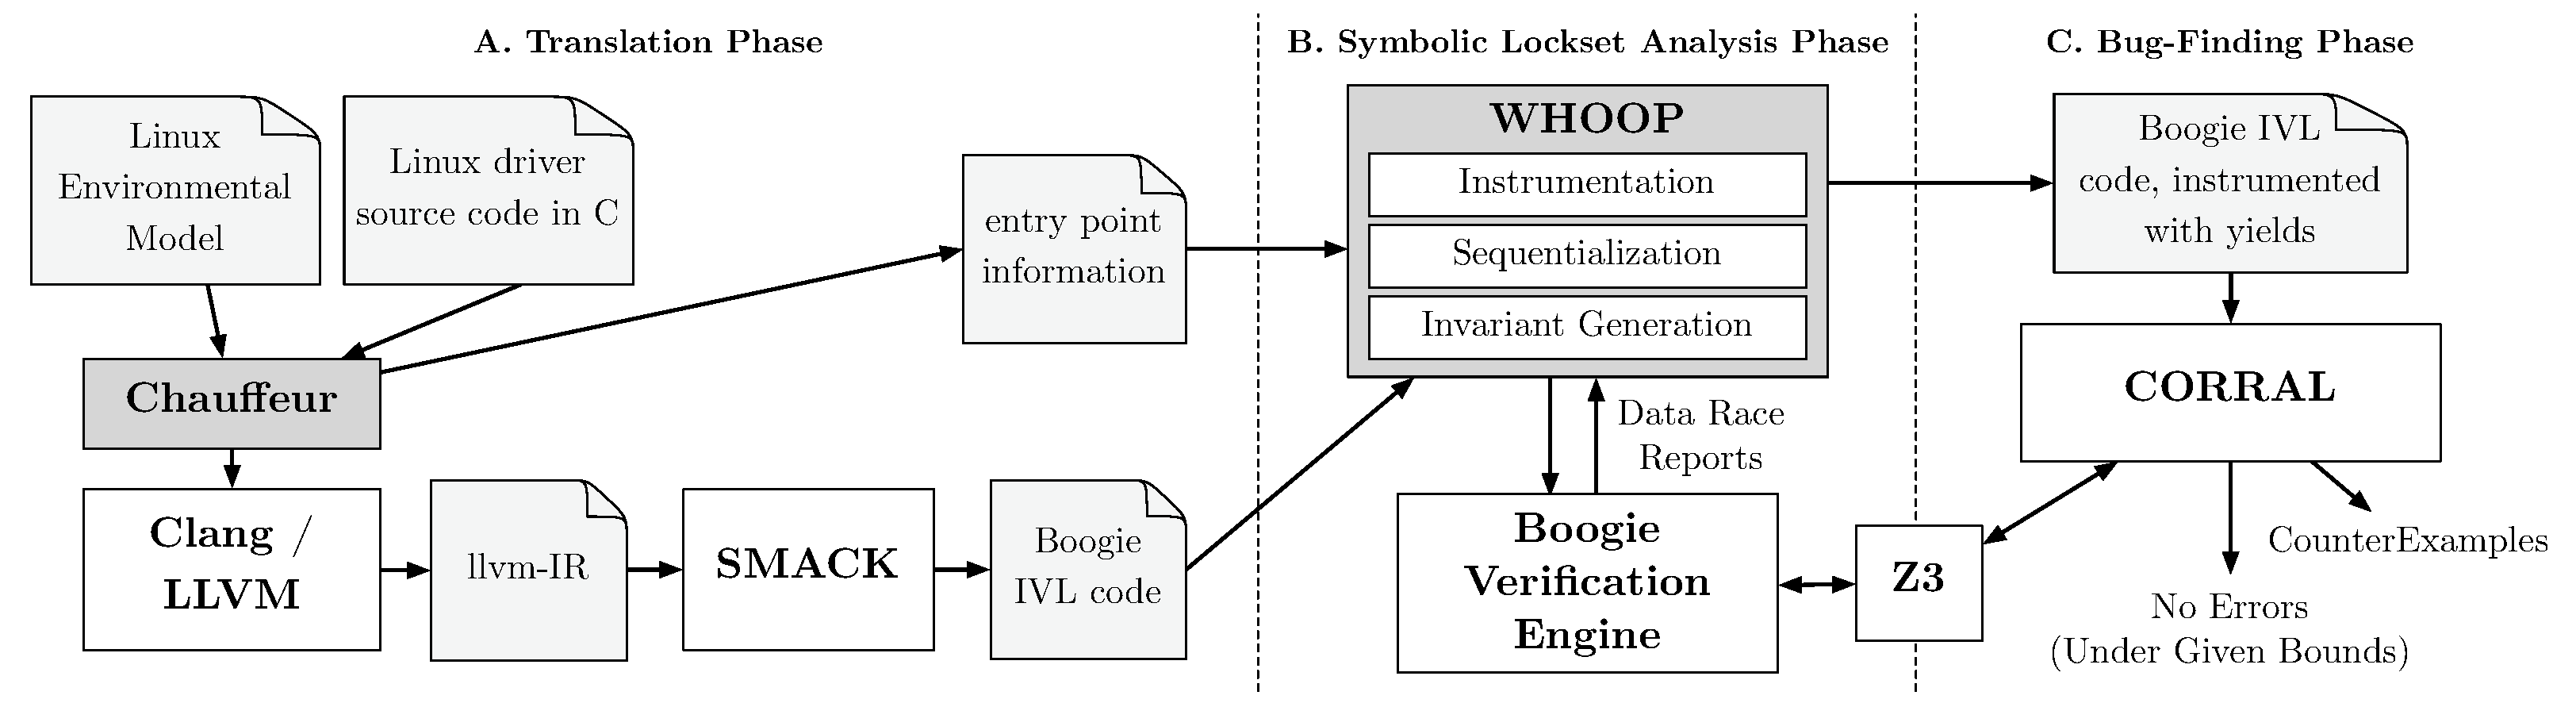
\includegraphics[width=.99\linewidth]{img/whoop.pdf}
\caption{The \whoop infrastructure, empowered by state-of-the-art compilation (Clang/LLVM and SMACK) and verification (Boogie and \corral) tools}
\label{fig:whoop}
\end{figure*}

The key idea behind our novel static analysis is that we can verify absence of data races by (i) deriving a sound \emph{sequential} model that \emph{over-approximates} the originally concurrent program, (ii) instrumenting it for lockset analysis and race-checking, and (iii) asserting that all write/read accesses to the same shared resource are consistently protected by at least one common lock. The immediate benefit is that our approach not only avoids reasoning about thread interleavings, and thus has the potential to scale well, but also allows the reuse of existing sequential verification techniques.

Figure~\ref{fig:whoop} depicts the \whoop toolchain. Initially, \whoop accepts a Linux driver written in C, together with a Linux environmental model\footnote{Stub header files that model the Linux kernel APIs.}, which is required to ``close'' the driver and allow it to be subsequently over-approximated and analyzed. Both the driver and the environmental model are passed to the translation phase of \whoop (see Section~\ref{whoop:translation}), which outputs an over-approximated program written in the Boogie intermediate verification language (IVL)~\cite{deline2005boogiepl}. Next, \whoop performs \emph{static pairwise lockset analysis} to detect all potential data races in the abstract program. The proof sketch behind our static lockset analysis is given in Section~\ref{whoop:proof}. The instrumentation and analysis is described in more detail in Section~\ref{whoop:method}. The summarization that we perform to achieve scalability is presented in Section~\ref{whoop:summarization}. After the static lockset analysis phase, \whoop exploits the race-related information to accelerate bug-finding with \corral (see Section~\ref{corral})

Finally, we discuss optimizations and assumptions in Section~\ref{whoop:optimizations}, and limitations of our technique in Section~\ref{whoop:limitations}.

\subsection{Translation to Boogie IVL}
\label{whoop:translation}

The aim of this phase (see Figure~\ref{fig:whoop} -- A) is to take an input Linux driver written in C, together with an environmental model, and output an over-approximated version of the program in Boogie IVL, a simple imperative language with well-defined verification-focused semantics used as the input to a number of cutting-edge verifiers (e.g. Boogie and \corral). To achieve this translation, \whoop uses three LLVM\footnote{\url{http://llvm.org}}-based tools: Chauffeur\footnote{\url{https://github.com/mc-imperial/chauffeur}}, Clang\footnote{\url{http://clang.llvm.org}} and SMACK\footnote{\url{https://github.com/smackers/smack}}~\cite{rakamaric2014smack}.

First, \whoop runs Chauffeur, a Clang-frontend that we developed to perform two tasks: (i) visit the abstract syntax tree (AST) of the original program and extract all available entry point identifier names in the given driver, together with the identifier names of their corresponding kernel callbacks; and (ii) instrument the original program with a function that calls all available entry points. This function acts as the main entry point to the driver after the latter has been registered with the kernel. This simple rewriting does not alter the semantics of the original program, is required so that Clang does not compile away any uncalled entry points (because we closed the environment using stub functions) and is also later used by \whoop to help instrument asynchronous calls to entry points and create checker procedures (see Sections~\ref{whoop:method} and~\ref{corral}). The output is a file that contains information regarding the entry points and a file with the rewritten program.

Next, the rewritten program is passed to Clang which compiles it to LLVM-IR~\cite{lattner2004llvm}, a low-level assembly-like language in single static assignment (SSA) form. SMACK then translates the LLVM-IR to Boogie IVL. SMACK leverages the pointer-alias analyses of LLVM to efficiently model the heap manipulation operations of the original program in Boogie IVL. To achieve scalability, SMACK is using a split-memory model instead of a monolithic one that would be difficult for backend verifiers to reason about~\cite{rakamaric2009scalable}.

\begin{lstlisting}[caption = Simple networking entry point in C, label = fig:original_program]
static void ep1(struct net_device *dev) {
  struct shared *tp = netdev_priv(dev);
  mutex_lock(&tp->wk.mutex);
  tp->resource = 4;
  mutex_unlock(&tp->wk.mutex);
}
\end{lstlisting}

Example~\ref{fig:original_program} shows a simple program in C and Example~\ref{fig:smack_translation} shows its corresponding translation in Boogie IVL using SMACK. The function \texttt{\$pa} models pointer arithmetic, while the map \texttt{\$M.0} is a memory region that typically denotes a shared resource. Notice that function calls (e.g. to lock and unlock a mutex) are preserved in the translation.

\begin{boogie}[caption = Translation to Boogie IVL using SMACK, label = fig:smack_translation]
procedure ep1(dev: int) modifies $M.0; {
  var $p0, $p1, $p2, $p3, $p4, $p5, $p6: int;
  $bb0:
    $p0 := dev;
    $p1 := $pa($p0, 32, 1);
    $p2 := $pa($pa($p1, 0, 24), 12, 1);
    $p3 := $pa($pa($p2, 0, 12), 0, 1);
    call mutex_lock($p3);
    $p4 := $pa($pa($p1, 0, 24), 4, 1);
    $M.0[$p4] := 4;
    $p5 := $pa($pa($p1, 0, 24), 12, 1);
    $p6 := $pa($pa($p5, 0, 12), 0, 1);
    call mutex_unlock($p6);
    return;
}
\end{boogie}

\subsection{Static Lockset Analysis Proof Sketch}
\label{whoop:proof}

We now formalize our approach to verifying data race freedom in a driver by statically analyzing its locksets. Let $\{\mathit{ep}_{1}, \mathit{ep}_{2}, \dotsc, \mathit{ep}_{n}\}$ be all the entry points of a driver, and let $\{\ell_{1}, \ell_{2}, \dotsc, \ell_{k}\}$ be all the locks used by this driver. Although we assume that the number of locks is finite and with a known bound, we argue that this assumption is realistic: all drivers that we have studied so far in the Linux kernel have only a small number of locks (typically one). Indeed, the Linux device driver book~\cite{corbet2005linux} advocates the use of as few locks as possible to avoid introducing unnecessary complexity and synchronization bugs that arise from careless fine-grained locking. Note that the actual Linux kernel employs sophisticated fine-grained locking, but this is part of the environment which is abstracted away in our models.

For each entry point $\mathit{ep}_{i}$, we compute its lockset $\mathit{LS}_{i}$ that associates each memory location $m$ to the set of locks that are always held when $m$ is accessed during the execution of $\mathit{ep}_{i}$. Furthermore, for each entry point $\mathit{ep}_{i}$, we compute its read-set $R_{i}\lbrack m\rbrack \rightarrow \{true, false\}$ and its write-set $W_{i}\lbrack m\rbrack \rightarrow \{true, false\}$, which map each $m$ to true if and only if $\mathit{ep}_{i}$ reads or writes respectively to $m$ during some execution. In the actual implementation we avoid the use of quantifiers by using a different lockset, read-set and write-set for each shared memory location.

\begin{theorem}
\label{theorem:locksets}
For each pair of entry points $\mathit{ep}_{i}, \mathit{ep}_{j}\in \{\mathit{ep}_{1}, \mathit{ep}_{2}, ..., \mathit{ep}_{n}\}$, where $i$ may be equal to $j$, and for each memory location $m$, if $(W_{i}\lbrack m\rbrack \vee W_{j}\lbrack m\rbrack) \wedge (W_{i}\lbrack m\rbrack \vee R_{j}\lbrack m\rbrack) \wedge (R_{i}\lbrack m\rbrack \vee W_{j}\lbrack m\rbrack) \implies (\mathit{LS}_{i}\lbrack m\rbrack \cap \mathit{LS}_{j}\lbrack m\rbrack \not= \varnothing)$, then the driver with entry points $\{\mathit{ep}_{1}, \mathit{ep}_{2}, \dotsc, \mathit{ep}_{n}\}$ is free from data races.
\end{theorem}

A sketch of how the above theorem can be proved is as follows. Suppose there are in fact entry points $\mathit{ep}_{i}$ and $\mathit{ep}_{j}$ that can race on a memory location $m$. By our hypothesis, there exists at least one lock, say $\ell$, which belongs to both $\mathit{LS}_{i}$ and $\mathit{LS}_{j}$. By the definition of a lockset, this means that $\ell$ is held during the access to $m$ by both $ep_1$ and $ep_2$. As a result, $m$ \emph{must} be unlocked and locked between the two accesses, which contradicts that the pair of accesses is racing.

\subsection{Instrumentation and Analysis}
\label{whoop:method}

The core \whoop tool (see Figure~\ref{fig:whoop} -- B) is responsible for parsing, instrumenting and sequentializing the abstract Boogie program. During the initial parsing, \whoop performs a static analysis (on the Boogie IVL code) to identify all lock identifiers and rewrite them to a unique constant Boogie variable, e.g. the following call to \texttt{mutex\_lock()}:

\begin{boogie}
call mutex_lock($p3);
\end{boogie}

Will be rewritten to:

\begin{boogie}
const {:lock} unique lock$0: int;
call mutex_lock(lock$0);
\end{boogie}

If \whoop cannot infer a lock it will exit with a warning. A limitation of lockset analysis is that it cannot understand external locking mechanisms (\whoop currently only supports Linux kernel mutexes and spinlocks). It is relatively straightforward to enhance \whoop, though, with new locking primitives. \whoop will also exit with a warning if it detects ``improper'' use of locks (e.g. dynamic lock creation). The reason behind this is twofold: first, it is arguably infeasible to detect such locks using static analysis; and second, because we want to advocate the use of good locking practices when developing drivers for the Linux kernel.

When the lock rewriting finishes, \whoop traverses the Boogie IVL code, uses the information extracted by Chauffeur and separates each independent entry point call-graph from the rest of the program. To achieve this, it duplicates helper functions and renames them accordingly: e.g. for entry point \texttt{ep1}, a helper function \texttt{foo} will be renamed to \texttt{foo\$ep1}. This allows \whoop to perform entry point sensitive instrumentation and analysis. Although the program can potentially become much larger, this does not affect the analysis as discussed later.

Next, \whoop instruments the program with global variables for lockset analysis and race-checking per entry point. For example, for entry point \texttt{ep1}, \whoop instruments:

\begin{boogie}
var {:current_lockset} lock$0_in_CLS_$ep1: bool;
var {:lockset} lock$0_in_LS_$M.0_$ep1: bool;
var {:access_checking} WRITTEN_$M.0_$ep1: bool;
var {:access_checking} READ_$M.0_$ep1: bool;
\end{boogie}

\whoop also instruments a global watchdog variable per memory region that is common to all entry points:

\begin{boogie}
const {:watchdog} WATCHED_ACCESS_$M.0: int;
\end{boogie}

The above instrumented variables represent the follows: \texttt{lock\$0\_in\_CLS\_\$ep1} is the current lockset (CLS) of \texttt{ep1}; \texttt{WATCHED\_ACCESS\_\$M.0} is an \emph{unconstrained} constant representing the offset to memory region \texttt{\$M.0} that should be checked for races; \texttt{lock\$0\_in\_LS\_\$M.0\_\$ep1} is the lockset for \texttt{\$M.0}; \texttt{WRITTEN\_\$M.0\_\$ep1} is the write-set for \texttt{\$M.0}; and \texttt{READ\_\$M.0\_\$ep1} is the read-set for \texttt{\$M.0}. Verification involves proving that two entry points cannot race at the watched offset of every memory region. The arbitrary watched offset implies that every offset of each memory region is race-free. Watchdog race-checking has been used before for verifying GPU kernels~\cite{bardsley2014engineering}.

\whoop proceeds by instrumenting each entry point call-graph for lockset analysis by replacing each call to a locking or unlocking function with a \whoop-specific lock and unlock functions. This means that Example~\ref{fig:smack_translation} will become:

\begin{boogie}
procedure ep1(dev: int) modifies $M.0; {
  var $p0, $p1, $p2, $p3, $p4, $p5, $p6: int;
  $bb0:
    $p0 := dev;
    $p1 := $pa($p0, 32, 1);
    $p2 := $pa($pa($p1, 0, 24), 12, 1);
    $p3 := $pa($pa($p2, 0, 12), 0, 1);
    call _UPDATE_CLS_$ep1(lock$0, true);
    $p4 := $pa($pa($p1, 0, 24), 4, 1);
    $M.0[$p4] := 4;
    $p5 := $pa($pa($p1, 0, 24), 12, 1);
    $p6 := $pa($pa($p5, 0, 12), 0, 1);
    call _UPDATE_CLS_$ep1(lock$0, false);
    return;
}
\end{boogie}

The \texttt{\_UPDATE\_CLS\_\$ep1()} is a special function that updates the CLS global variable to either true or false, if the lock is held or released by \texttt{ep1} accordingly:

\begin{boogie}
procedure {:inline 1} _UPDATE_CLS_$ep1(lock: int,
    isLocked: bool);
  modifies lock$0_in_CLS_$ep1;

implementation {:inline 1} _UPDATE_CLS_$ep1(
    lock: int, isLocked: bool) {
  _UPDATE:
    lock$0_in_CLS_$ep1 := (if lock == lock$0 then
      isLocked else lock$0_in_CLS_$ep1);
  return;
}
\end{boogie}

Next, \whoop replaces every write and read access in each entry point call-graph with a \whoop-specific function:

\begin{boogie}
procedure ep1(dev: int) modifies $M.0; {
  var $p0, $p1, $p2, $p3, $p4, $p5, $p6: int;
  $bb0:
    $p0 := dev;
    $p1 := $pa($p0, 32, 1);
    $p2 := $pa($pa($p1, 0, 24), 12, 1);
    $p3 := $pa($pa($p2, 0, 12), 0, 1);
    call _UPDATE_CLS_$ep1(lock$0, true);
    $p4 := $pa($pa($p1, 0, 24), 4, 1);
    call _WRITE_LS_$M.0_$ep1($p4);
    $p5 := $pa($pa($p1, 0, 24), 12, 1);
    $p6 := $pa($pa($p5, 0, 12), 0, 1);
    call _UPDATE_CLS_$ep1(lock$0, false);
    return;
}
\end{boogie}

The \texttt{\_WRITE\_LS\_\$M.0\_\$ep1()} is a special function that computes the intersection of the CLS and the lockset of \texttt{\$M.0} (see Section~\ref{bg:lockset}). It also updates the write-set of \texttt{\$M.0} to true, because there was a write access by \texttt{ep1}:

\begin{boogie}
procedure {:inline 1} _WRITE_LS_$M.0_$ep1(
    ptr: int);
  modifies lock$0_in_LS_$M.0_$ep1,
    WRITTEN_$M.0_$ep1;

implementation {:inline 1} _WRITE_LS_$M.0_$ep1(
    ptr: int) {
  _WRITE:
    goto anon1_Then, anon1_Else;

  anon1_Then:
    assume {:partition} WATCHED_ACCESS_$M.0 ==
      ptr && DEVICE_IS_REGISTERED_$ep;
    lock$0_in_LS_$M.0_$ep := lock$0_in_CLS_$ep && lock$0_in_LS_$M.0_$ep;
    WRITTEN_$M.0_$ep := true;
    return;
  anon1_Else:
    assume {:partition} !(WATCHED_ACCESS_$M.0 ==
      ptr && DEVICE_IS_REGISTERED_$ep);
    return;
}
\end{boogie}

The \texttt{\_READ\_LS\_\$M.0\_\$ep1()} updates the lockset of \texttt{\$M.0} and the read-set accordingly for a read access.

\whoop continues by performing \emph{two-thread reduction}, a sound abstraction that removes all but two arbitrary threads, each running an entry point of the originally concurrent program, and then performs \emph{pairwise sequentialization}, which combines the two arbitrary threads in a single sequential pair. This is achieved by creating a checker function that calls the two instrumented entry points and then performs race-checking assertions. This process repeats until all possible pairs of entry points have been sequentialized. To be sound, each time an entry point performs a read access to a shared memory location, \whoop returns a nondeterministic value (using the Boogie keyword \texttt{havoc}). This over-approximates any effects from all the unmodeled threads on the shared state of the pair. Two-thread reduction is not a new idea, it has been used before in GPU kernel verification~\cite{bardsley2014engineering} and in model checking of cache coherence protocols~\cite{mcmillan1999verification}.

After each checker function calls a pair of entry points, it asserts that each shared memory location is protected by at least one common lock (see Section~\ref{bg:lockset}). The assertion check is triggered iff the memory location was accessed by both entry points and at least one of the accesses was a write. We do not check for read-read races, which are inherently benign. The following is an example of a checker function for entry points \texttt{ep1} and \texttt{ep2}:

\begin{boogie}
procedure check$ep1$ep2(dev: int);
  requires !lock$0_in_CLS_$ep1;
  requires !lock$0_in_CLS_$ep2;
  requires lock$0_in_LS_$M.0_$ep1;
  requires lock$0_in_LS_$M.0_$ep2;
  requires !WRITTEN_$M.0_$ep1;
  requires !WRITTEN_$M.0_$ep2;
  requires !READ_$M.0_$ep1;
  requires !READ_$M.0_$ep2;
  modifies lock$0_in_CLS_$ep1, lock$0_in_CLS_$ep2,
    lock$0_in_LS_$M.0_$ep1, lock$0_in_LS_$M.0_$ep2,
    WRITTEN_ $M.0_$ep1,WRITTEN_$M.0_$ep2,
    READ_$M.0_$ep1, READ_$M.0_$ep2;

implementation check$ep1$ep2(dev: int) {
  _CHECK:
    call ep1(dev);
    call ep2(dev);
    assert (WRITTEN_$M.0_$ep1 && WRITTEN_$M.0_$ep2)
      || (WRITTEN_$M.0_$ep1 && READ_$M.0_$ep2)
      || (READ_$M.0_$ep1 && WRITTEN_$M.0_$ep2)
      ==> lock$0_in_LS_$M.0_$ep1 &&
      lock$0_in_LS_$M.0_$ep2;
    return;
}
\end{boogie}

Finally the abstract program is send to the Boogie verification engine, which generates verification conditions~\cite{barnett2005weakest} and discharges them to the Z3~\cite{de2008z3} theorem prover. Successful verification implies that the original program is free of data races, while an error denotes a \emph{potential} data race and is reported to the user. To improve usability, \whoop has a built-in error reporter that matches counterexamples to source code. The following is an example of a reported error:

\begin{lstlisting}
foo.c: error: potential write-write race:
  write by entry point ep1, foo.c:36:2
    shared->resource = 4;
  write by entry point ep2, foo.c:52:2
    shared->resource = 5;
\end{lstlisting}

\subsection{Watchdog Summarization}
\label{whoop:summarization}

Early on during the development of \whoop, we realized that scalability would be a serious issue. When we tried to apply \whoop on the r8169 RealTek ethernet driver (8000 lines of C code) with all functions fully inlined, we were running out of memory. One reason was that the C to Boogie translation produced hundreds of thousands of Boogie IVL code, which could not fit in memory. Another reason was that some entry points recursively call helper functions. Inherently, recursion does not work with inlining. To tackle these issues we developed \emph{watchdog summarization}, a novel summarization technique that allows us to analyze Linux drivers in a scalable fashion, but without destroying precision.

Watchdog summarization uses the Houdini~\cite{flanagan2001houdini} invariant inference algorithm (available inside Boogie) to automatically compute summaries (pre- and post-conditions and loop invariants) from a pool of \emph{candidate} invariants. The reason we need loop invariants is that we over-approximate loops using loop-cutting (also available inside Boogie).

The candidate invariants are based on the global variables that \whoop instruments to perform lockset analysis and race-checking (see Section~\ref{whoop:method}). The key idea behind watchdog summarization is that we automatically generate candidate invariants for each memory region in the granularity of watched accesses. This reduces the false positives from reporting errors if only e.g. a field in memory region \texttt{\$M.0} is racing, but the rest of the fields are not. An example of watchdog-based candidate post-conditions is the following:

\begin{boogie}
procedure foo$ep1(dev: int);
  ensures _b$ls$entrypoint1$0
    ==> WATCHED_ACCESS_$M.0 == dev + 4
    ==> lock$0_in_LS_$M.0_$entrypoint1;
  ensures _b$ls$entrypoint1$1
    ==> WATCHED_ACCESS_$M.0 == dev + 8
    ==> lock$0_in_LS_$M.0_$entrypoint1;
  ensures _b$ac$entrypoint1$0
    ==> WATCHED_ACCESS_$M.0 == dev + 4
    ==> !WRITTEN_$M.0_$entrypoint1;
  ensures _b$ac$entrypoint1$1
    ==> WATCHED_ACCESS_$M.0 == dev + 8
    ==> !WRITTEN_$M.0_$entrypoint1;
  ...
\end{boogie}

To generate the candidate invariants, \whoop performs an intra-procedural static analysis on the call-graph (in Boogie IVL code) of each entry point, identifying all possible accesses to shared memory locations. To be sound, if \whoop cannot infer information for a specific access, it generates a coarse-grained candidate for the corresponding memory region. For example the previous \texttt{\$M.0} candidates would now be:

\begin{boogie}
procedure foo$ep1(dev: int);
  ensures _b$ls$entrypoint1$0
    ==> lock$0_in_LS_$M.0_$entrypoint1;
  ensures _b$ls$entrypoint1$1
    ==> lock$0_in_LS_$M.0_$entrypoint1;
  ensures _b$ac$entrypoint1$0
    ==> !WRITTEN_$M.0_$entrypoint1;
  ensures _b$ac$entrypoint1$1
    ==> !WRITTEN_$M.0_$entrypoint1;
  ...
\end{boogie}

\subsection{Optimizations and Assumptions}
\label{whoop:optimizations}

To increase precision we enhance \whoop with domain-specific knowledge of how the Linux kernel interacts with its drivers. This is an ongoing manual effort: the more drivers we study, the more domain-specific properties we discover, which we then exploit to make \whoop more precise.

In our experience, one of the most effective precision optimizations is to enrich \whoop with information regarding kernel-imposed serialization. The Linux kernel can serialize calls to entry points, thus forcing them to not run concurrently with each other. An an example, a large number of networking and ethernet entry points are mutually serialized with RTNL, a network-specific kernel lock. \whoop exploits this knowledge and does not create pairs for entry points that are serialized.

Modeling kernel methods is another opportunity to increase precision, but requires Linux kernel expertise. For example, the \texttt{register\_netdev()} function registers a network driver with the kernel. Before this function is called, the kernel is not able to invoke any of the driver's entry points. Modeling this functionality can reduce false positives when race-checking accesses before the driver's registration.

Another optimization \whoop uses is to soundly reduce the checked memory locations. If a memory location is accessed only by one entry point in a pair, then it is safe to not check this location for this pair. This reduces the burden to the SMT solver and speed up the verification process.

%We also optimize the use of function pointers. LLVM and SMACK do not perform context-sensitive translation, which means that a function that accepts a function pointer as an argument, can arbitrarily call any possible method that corresponds to that function pointer regardless of call site. To increase precision, Chauffeur analyses the AST of the original program and attempts to infer context-sensitive function pointer use information. This information is the used by \whoop to increase precision. To be sound, this optimization is conservative: if no information can be extracted for a function pointer at a call site, then \whoop uses the original over-approximated function.

Finally, we assume that the formal parameters of an entry point do not alias, and thus cannot race. This is a potentially unsound feature that can be turned off using a command line option. In our experience so far, though, we have not missed any data races because of this assumption. We also assume that our environmental model and domain-specific knowledge are correct and do not cause any bugs to be missed.

\subsection{Limitations}
\label{whoop:limitations}

\whoop is based on lockset analysis and thus can report false bugs, because a violation of the locking discipline does not always correspond to a real data race (e.g. when lockfree synchronization is used instead of locking). \whoop also uses over-approximation (e.g. when reading from the shared state) and summarization, which can be sources of false positives. Furthermore, the tool does not currently check for dynamically created locks or for locks that are provided by external libraries, although the later could be addressed by providing a mechanism for users to declare custom locks.

Another limitation of \whoop is that it is unable to verify drivers that are designed to be accessed by a single process at a time. This \emph{single-open device}~\cite{corbet2005linux} mode can be enforced by atomically testing (at the beginning of each entry point) a flag that indicates device availability: if the flag is set to true, then the respective entry point executes, else it blocks. Because \whoop performs pair-wise analysis, it over-approximates this flag, and regards a pair of entry points as running concurrently, even if this is not the case. However,~\cite{corbet2005linux} advises against serializing drivers in this way, as it hinders user ingenuity (e.g. a user might expect that a device can be accessed concurrently for performance). Because using single-open device mode is considered bad practice, we thus burden the developer with disregarding any related false bug reports.

Statically analyzing system-level software, such as drivers, requires to ``close'' the environment by abstracting away the low level implementation details. In this work, we developed a simple environmental model for the Linux kernel that consists of (nondeterministic) stub functions. A limitation of our model is that it can, and will, ultimately result in decreased precision and, thus, false positives. However, because we currently only focus on finding data races, we can get away with over-approximating a lot of the underlying Linux kernel functionality, without losing too much precision. Enriching our model with domain-specific knowledge to make it more precise is an ongoing manual effort, but requires Linux expertise. We argue that further increasing the precision is orthogonal to the contributions of this paper. Moreover, even if the symbolic lockset analysis results in false positives, \whoop can still use any race-freedom guarantees to significantly speedup a more precise bug-finder, as seen in Sections~\ref{corral} and~\ref{evaluation}.
